\documentclass{beamer}
\usepackage{times}
\usepackage{tikz}
\usepackage{beamerthemesplit}
\usetheme{Antibes}
\usepackage{tcolorbox}

\title{The Security Framework of White-Box Cryptography Revisited}
\author{Yufeng Tang, Tao Sun, Zheng Gong\\ \url{cis.gong@gmail.com}}
\institute{\inst{1}{School of Computer Science, South China Normal University} \\ \inst{2}{Mobile Applications And Security Engineering Center of Guangdong Province}}

\date{\today}

\begin{document}

\frame
{
 \titlepage
}

\section[Outline]{}
\frame{\tableofcontents}

\section{White-box cryptography: background}
\frame{
\frametitle{Cryptography: the very beginning}
"Information theory is about communication in the presence of noise."
\begin{flushright}
-C. Shannon, 1948.\footnote{\scriptsize{\url{http://fab.cba.mit.edu/classes/S62.12/docs/Shannon_noise.pdf}}}
\end{flushright}

\begin{center}
\begin{tikzpicture}
    \node[anchor=south west,inner sep=0] (image) at (0,0) { 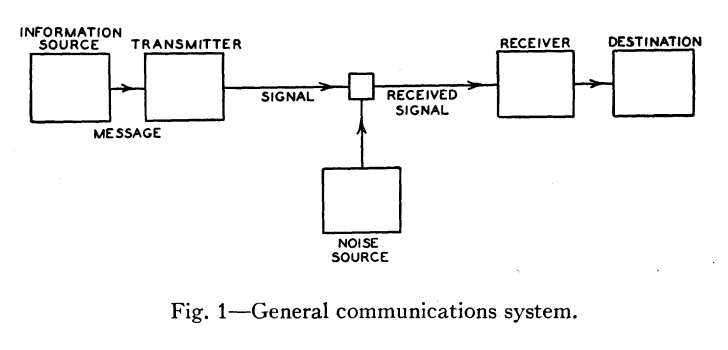
\includegraphics[width=8cm, height=4cm]{./pics/Shannon_GeneralCommunicationSystem.png}};

    %\begin{scope}[x={(image.south east)},y={(image.north west)}]
        %\draw[help lines,xstep=.1,ystep=.1] (0,0) grid (1,1);
        %\foreach \x in {0,1,...,9} { \node [anchor=north] at (\x/10,0) {0.\x}; }
        %\foreach \y in {0,1,...,9} { \node [anchor=east] at (0,\y/10) {0.\y}; }
        %\draw[green, ultra thick, rounded corners] (0.24,0.18) rectangle (0.50,0.32);
    %\end{scope}
\end{tikzpicture}
\end{center}
}

\frame{
\frametitle{Cryptography: an informal definition}
"Cryptography is about communication in the presence of adversaries."
\begin{flushright}
-R. Rivest
\end{flushright}

\begin{center}
\begin{tikzpicture}
    \node[anchor=south west,inner sep=0] (image) at (0,0) { 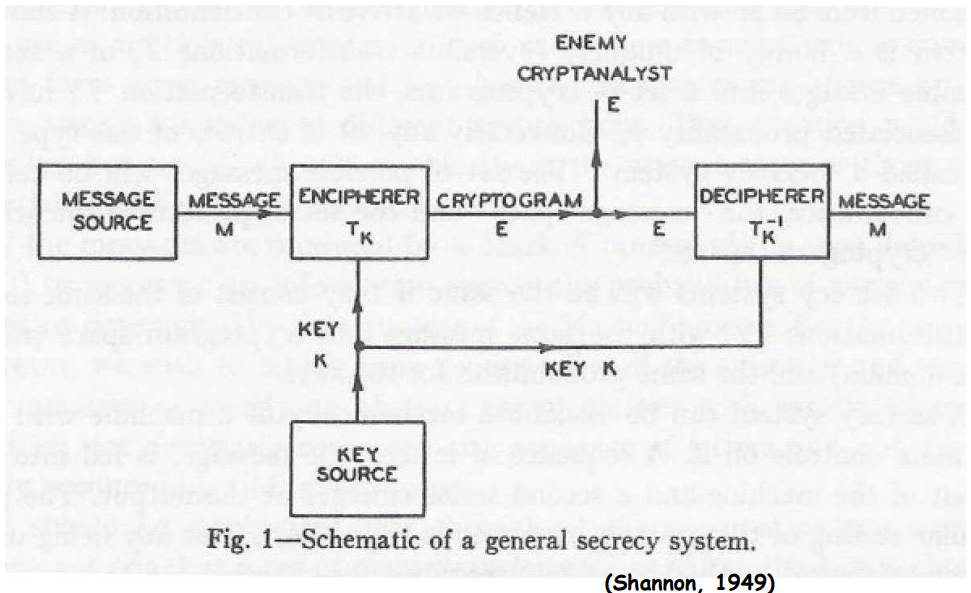
\includegraphics[width=8cm, height=5cm]{./pics/Shannon_GeneralSecrecySystem.png}};

    %\begin{scope}[x={(image.south east)},y={(image.north west)}]
        %\draw[help lines,xstep=.1,ystep=.1] (0,0) grid (1,1);
        %\foreach \x in {0,1,...,9} { \node [anchor=north] at (\x/10,0) {0.\x}; }
        %\foreach \y in {0,1,...,9} { \node [anchor=east] at (0,\y/10) {0.\y}; }
        %\draw[green, ultra thick, rounded corners] (0.24,0.18) rectangle (0.50,0.32);
    %\end{scope}
\end{tikzpicture}
\end{center}
}

\frame{
\frametitle{Define cryptography in ``a mathematically acceptable way"}
\textcolor{red}{``As a first step in the mathematical analysis of cryptography, it is necessary to idealize the situation suitably, and to define in a mathematically acceptable way what we shall mean by a secrecy system."}

\begin{flushright}
-C. Shannon, 1949. \footnote{{\scriptsize``Communication Theory of Secrecy Systems", Bell System Tech. J., vol. 28, pp. 656-715, Oct., 1949.}}
\end{flushright}
}

\frame
{
\frametitle{The Kerckhoffs' principle of cryptography}

\begin{columns}[c]
\column{.65\textwidth}
A cipher should be secure when the enemy cryptanalyst knows all details of the enciphering process and deciphering process except for the value of the secret key.

\begin{flushright}
- stated in 1881 by the Dutchman Auguste Kerckhoffs (1835-1903).
\end{flushright}
\begin{itemize}
\setlength{\itemsep}{12pt}
%\item Do not rely on keeping an algorithm secret.
%\item Publish an algorithm but keep the key secretly.
\item \textcolor{red}{Have some mathematical foundation for the belief that it will be hard to extract the key.}
\end{itemize}

\column{.35\textwidth}
\begin{figure}[htbp]
\centering
  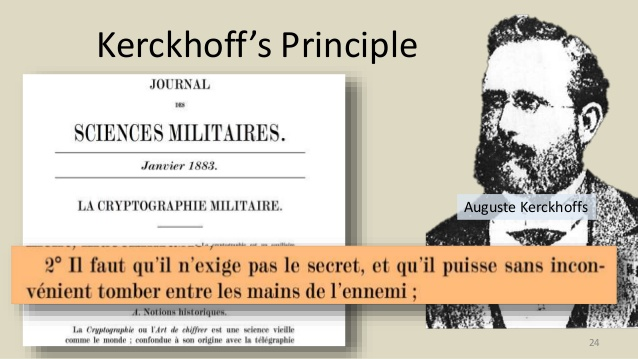
\includegraphics[width=4cm, height=3cm]{./pics/Kerckhoffs.jpg}
\end{figure}

\end{columns}
}

%\frame{
%\frametitle{The Kerckhoffs' principle of a secrecy system}
%A cipher should be secure when the enemy cryptanalyst knows all details of the enciphering process and deciphering process except for the value of the secret key.
%
%\begin{flushright}
%- stated in 1881 by the Dutchman Auguste Kerckhoffs (1835-1903).
%\end{flushright}
%
%
%\begin{center}
%\begin{tikzpicture}
%    \node[anchor=south west,inner sep=0] (image) at (0,0) { 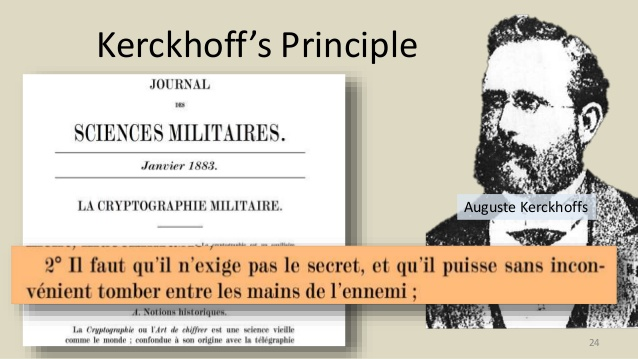
\includegraphics[width=6cm, height=4cm]{./pics/Kerckhoffs.jpg}};
%
%    %\begin{scope}[x={(image.south east)},y={(image.north west)}]
%        %\draw[help lines,xstep=.1,ystep=.1] (0,0) grid (1,1);
%        %\foreach \x in {0,1,...,9} { \node [anchor=north] at (\x/10,0) {0.\x}; }
%        %\foreach \y in {0,1,...,9} { \node [anchor=east] at (0,\y/10) {0.\y}; }
%        %\draw[green, ultra thick, rounded corners] (0.24,0.18) rectangle (0.50,0.32);
%    %\end{scope}
%\end{tikzpicture}
%\end{center}
%}

\frame{
\frametitle{The goal of modern cryptography}
\begin{itemize}
\item The goal of modern cryptography is to design, analysis, and implement a cryptosystem which obtains a mathematically acceptable security proofs.

\begin{itemize}
\item Confidentiality / Secrecy
\item Integrity
\item Authenticity
\item Availability
\end{itemize}

\item Thus provable security must be reduced on \textcolor{red}{an acceptable model!}
\begin{itemize}
\item Ideal cipher model
\item Random oracle model/Standard model
\item Indifferentiability model
\end{itemize}
\end{itemize}
}

\frame{
\frametitle{How to modeling attackers in cryptography}
\begin{center}
\begin{tikzpicture}
    %\node[anchor=south west,inner sep=0] (image) at (0,0) { 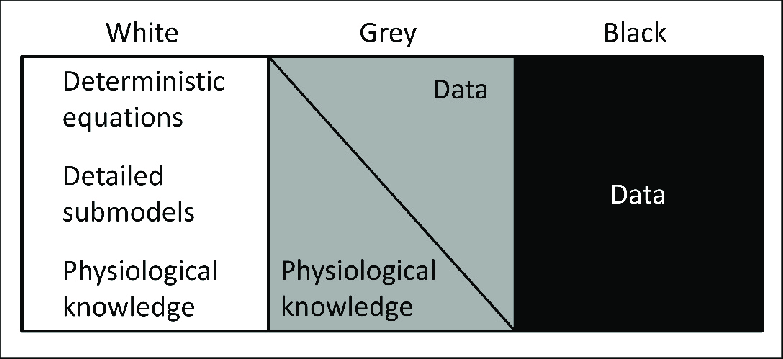
\includegraphics[width=6cm, height=4cm]{./pics/Illustration-of-the-concept-of-Black-White-Grey-box-modeling.png}};
    \node[anchor=south west,inner sep=0] (image) at (0,0) { 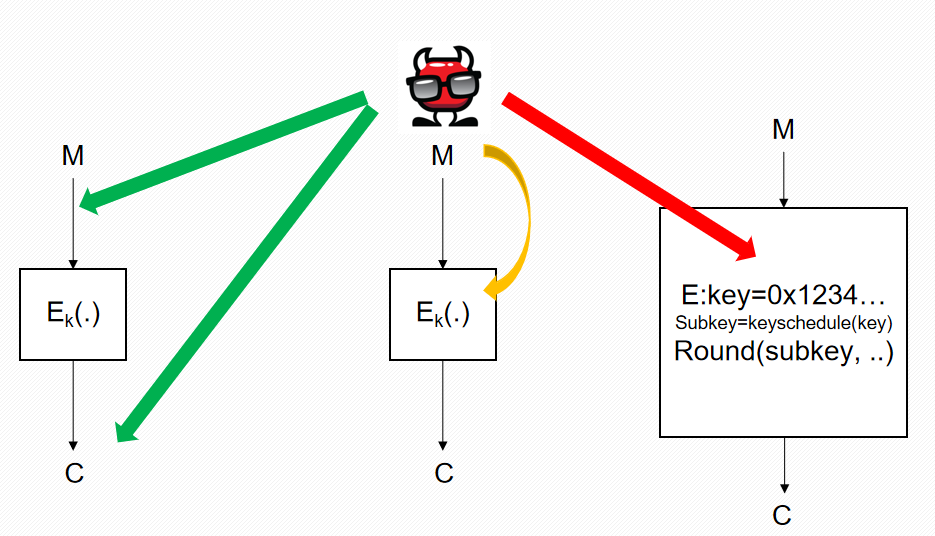
\includegraphics[width=7cm, height=4cm]{./pics/WBC_Model.png}};

    %\begin{scope}[x={(image.south east)},y={(image.north west)}]
        %\draw[help lines,xstep=.1,ystep=.1] (0,0) grid (1,1);
        %\foreach \x in {0,1,...,9} { \node [anchor=north] at (\x/10,0) {0.\x}; }
        %\foreach \y in {0,1,...,9} { \node [anchor=east] at (0,\y/10) {0.\y}; }
        %\draw[green, ultra thick, rounded corners] (0.24,0.18) rectangle (0.50,0.32);
    %\end{scope}
\end{tikzpicture}
\end{center}
}

\section{The security framework of WBC}
\subsection{Basic concepts of modeling}
\frame{
\frametitle{Black-box model}
\begin{itemize}
\item The adversary is able to know, choose or adaptively choose inputs and outputs of the function.

\item Given the black-box implementation of the function, the adversary aims to \textcolor{red}{recover the secret values} or to \textcolor{orange}{misbehave the function}.
\end{itemize}
}

\frame{
\frametitle{White-box model}
\begin{itemize}
\item Informally speaking, an adversary in \textcolor{red}{white-box model} can tamper, modify, manipulate all intermediate values and processes of the implementation of a secrecy system.
\item It can be looked as a superset of \textcolor{red}{black-box} and \textcolor{red}{grey-box} models.
\end{itemize}
}

\frame{
\frametitle{Grey-box model}
According to the black/white-box modeling, the grey-box adversary is able to
\begin{itemize}
\item know, choose or adaptively choose inputs and outputs of the function;

\item tamper, modify, manipulate intermediate values with specific (physical) knowledge.

\end{itemize}
}

\frame{
\frametitle{An illustration of the Black/White/Grey-box modeling}
\begin{center}
\begin{tikzpicture}
    \node[anchor=south west,inner sep=0] (image) at (0,0) { 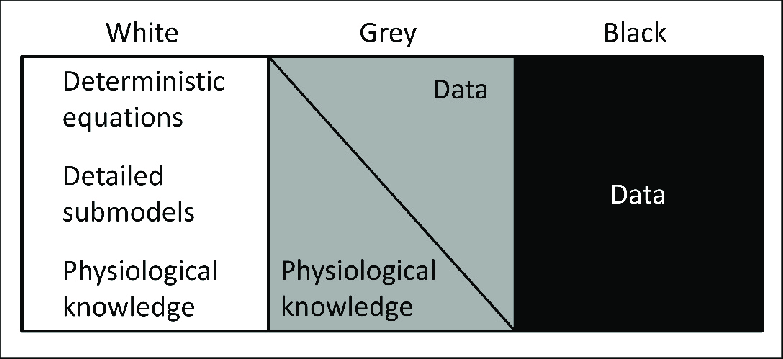
\includegraphics[width=9cm, height=4cm]{./pics/Illustration-of-the-concept-of-Black-White-Grey-box-modeling.png}};
    %\node[anchor=south west,inner sep=0] (image) at (0,0) { 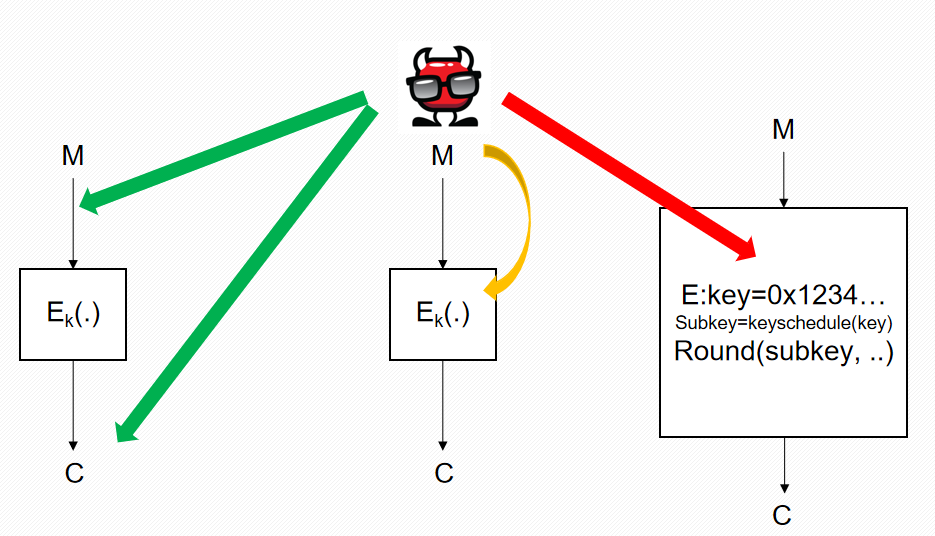
\includegraphics[width=7cm, height=4cm]{./pics/WBC_Model.png}};

    %\begin{scope}[x={(image.south east)},y={(image.north west)}]
        %\draw[help lines,xstep=.1,ystep=.1] (0,0) grid (1,1);
        %\foreach \x in {0,1,...,9} { \node [anchor=north] at (\x/10,0) {0.\x}; }
        %\foreach \y in {0,1,...,9} { \node [anchor=east] at (0,\y/10) {0.\y}; }
        %\draw[green, ultra thick, rounded corners] (0.24,0.18) rectangle (0.50,0.32);
    %\end{scope}
\end{tikzpicture}
\end{center}
}

\frame
{
\frametitle{A typical white-box block cipher in a nutshell}
\begin{figure}[htbp]
\centering
  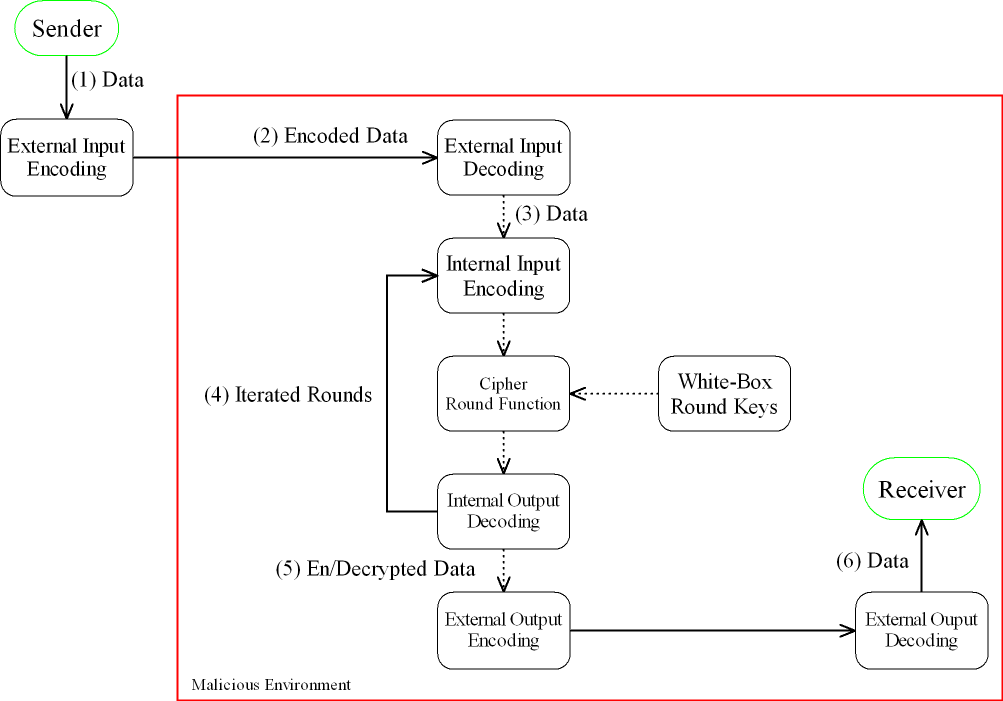
\includegraphics[width=8cm]{./pics/WBCrypto_Functional_Model.png}

\end{figure}

}

\frame
{
 \frametitle{WBC Implementations of DES/AES/SM4/... (All broken!)}
 \begin{itemize}
  \item Chow \textit{et al.} Tbox-based WBDES/AES, 2002
  \item Link and Neumann. Tbox-based WBTDES, 2005
  \item Bringer. Isomorphism of Polynomials, WBAES, 2006
  \item Xiao and Lai. 16-bit Tbox WBAES, 2009
  \item Xiao and Lai. Affine-function WBSM4, 2009
  \item Karroumi \textit{et al.} Dual-cipher WBAES, 2011
  \item Shi \textit{et al.} Tbox-based WBSHARK, 2013
  \item Luo \textit{et al.} ShiftRows table WBAES, 2014
  \item Su \textit{et al.} Random number WBCLEFIA, 2014
  \item Shi \textit{et al.} Dual-cipher WBSM4, 2015
  \end{itemize}
}

\frame
{
 \begin{itemize}
  \item Baek \textit{et al.} Larger Tbox WBAES, 2016
  \item Bai and Wu. Uncombinable encodings WBSM4, 2016
  \item Lee \textit{et al.} Masked WBAES, 2018
  \item Xu \textit{et al.} Obfuscated round boundaries WBAES/SM4, 2018
  \item Bai \textit{et al.} Affine-function WBAES, 2018
  \item Zhou \textit{et al.} Lightweight WBC, 2018
  \item Lv \textit{et al.} WB-KMAC, 2019
  \item Lee and Kim. Table redundancy WBAES, 2019
  \item Lee and Kim. Improved masked WBAES, 2020
  \item Yao and Chen. Random state WBSM4, 2020
  \item Yao \textit{et al.} Affine-function WBCLEFIA, 2020
  \item Yao \textit{et al.} Affine-function WBGIFT, 2021
 \end{itemize}
}

\frame
{
 \frametitle{Dedicated WBC Proposals}
 \begin{itemize}
  \item Biyukov \textit{et al.} ASASA structure, 2014
  \item Bogdanov and Isobe. SPACE, 2015
  \item Bogdanov and Isobe. SPNbox, 2016
  \item Fouque \textit{et al.} WhiteBlock, 2016
  \item Bai and Wu. AES-Like cipher, 2016
  \item Cho and Dinur. WEM, 2017
  \item Lin \textit{et al.} ASASASA structure, 2017
  \item Xu \textit{et al.}. AES-like cipher, 2017
  \item Shi \textit{et al.} SDSRS, 2020
  \item Kwon \textit{et al.} FPL, 2020
  \item Koike \textit{et al.} Galaxy, 2020
 \end{itemize}
}

\subsection{The proposed security notions and their problems}
%
%\frame{
%\frametitle{Chow \textit{et al.}'s definitions}
%In Chow \textit{et al.}'s seminal work on white-box AES implementations, they proposed some basic notions intuitively.
%\begin{itemize}
%\item White-box attack context
%\item White-box s
%\item White-box security metrics
%
%\end{itemize}
%}

\frame{
\frametitle{Basic security definitions for WBC}
\begin{definition}(\textcolor{red}{Secret key recovery (KR-Security)}). A white-box implementation of a key-instantiated block cipher $E_{k}$ (or $D_{k}$) is called \textit{KR-insecure} if an attacker extracts the secret key $k$ and furthermore has access to the plaintext $P$.
\end{definition}

\begin{definition}
(\textcolor{red}{White-box key recovery (WBKR-Security)}). A white-box implementation of an encoded version of a key-instantiated block cipher $E_{k}$ (or $D_{k}$) is called \textit{WBKR-insecure} if the attacker extracts the secret key $k$ and the inverse mappings of the applied external encodings.
\end{definition}
}

\frame{
\frametitle{Basic security definitions for WBC (Chow \textit{et al.})}
\begin{itemize}
\item In SAC 2002, the security notions have  been informally described for white-box cryptography by Chow \textit{et al.}. First the key recovery problem is informally defined by \textcolor{red}{the weak white-box security} (which equals to \textcolor{red}{KR-Security})
\end{itemize}

\begin{center}
\begin{tikzpicture}
    \node[anchor=south west,inner sep=0] (image) at (0,0) { 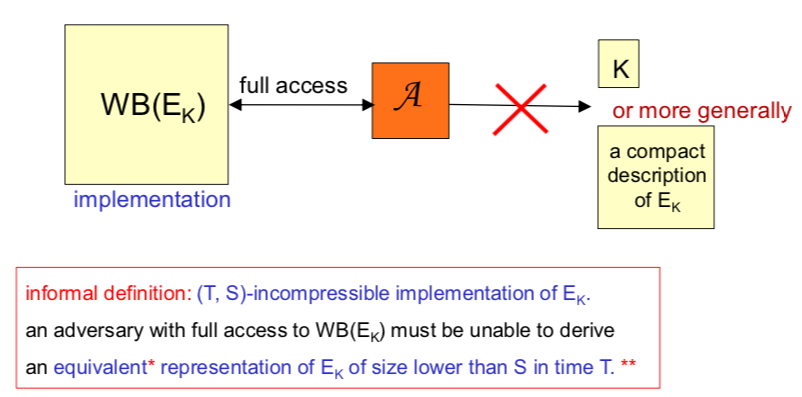
\includegraphics[width=8cm, height=4cm]{./pics/weak_white_box_security.png}};

    \begin{scope}[x={(image.south east)},y={(image.north west)}]
        %\draw[help lines,xstep=.1,ystep=.1] (0,0) grid (1,1);
        %\foreach \x in {0,1,...,9} { \node [anchor=north] at (\x/10,0) {0.\x}; }
        %\foreach \y in {0,1,...,9} { \node [anchor=east] at (0,\y/10) {0.\y}; }
        \draw[red, thin, rounded corners] (0.85,0.7) circle (1.2cm);
    \end{scope}
\end{tikzpicture}
\end{center}
}

\frame{
\frametitle{Basic security definitions for WBC (Biryukov \textit{et al.})}
\begin{itemize}
\item For more general security, \textcolor{red}{the strong white-box security} has been defined by [Biryukov \textit{et al.} 2014] (which connects to \textcolor{red}{KR/WBKR-Security})
\end{itemize}

\begin{center}
\begin{tikzpicture}
    \node[anchor=south west,inner sep=0] (image) at (0,0) { 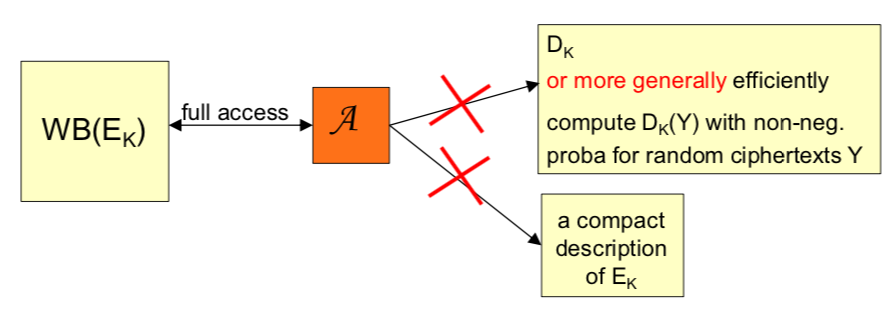
\includegraphics[width=10cm, height=4cm]{./pics/strong_white_box_security.png}};

    %\begin{scope}[x={(image.south east)},y={(image.north west)}]
        %\draw[help lines,xstep=.1,ystep=.1] (0,0) grid (1,1);
        %\foreach \x in {0,1,...,9} { \node [anchor=north] at (\x/10,0) {0.\x}; }
        %\foreach \y in {0,1,...,9} { \node [anchor=east] at (0,\y/10) {0.\y}; }
        %\draw[green, ultra thick, rounded corners] (0.24,0.18) rectangle (0.50,0.32);
    %\end{scope}
\end{tikzpicture}
\end{center}
}


\frame{
\frametitle{The problems of the weak/strong white-box security}
\begin{itemize}
\item It only works for white-box encryption/decryption, while does not suitable for \textcolor{red}{MAC/signature}.

\item ``A \textcolor{red}{compact} description of $E_{k}$/$/D_{k}$", it is very hard to measure security under this informal definition.
\end{itemize}
}

\frame{
\frametitle{The negative results on virtual black-box property (VBBP)}
\begin{itemize}
\item At Crypto 2001, Barak \textit{et al.} provided an insight on the impossibility of code obfuscation for \textcolor{red}{generic programs}.
\item \textcolor{red}{The virtual black-box property (VBBP)} has been proposed for defining the ideal code/program obfuscation.
\item The negative results are given by counterexamples that cannot satisfy the virtual black-box property (VBBP) in any circumstance.
\end{itemize}
}

\frame{
\frametitle{Recall the definitions of VBBP [Saxena2009] (1)}
\textbf{Correctness.}{$\mathcal{O}$ is an obfuscator for a polynomial time function $Q$ if the follow properties hold.}
\begin{enumerate}

\item \textit{(\textcolor{red}{Functionality})}. $\forall k, \forall (q,a)\in \mathcal{K}^{k}_{Q}\times \mathcal{I}^{k}_{Q}:\textmd{Pr}[\mathcal{O}(Q,k)(a) \neq Q [k](a)]\leq negl(k)$

\item \textit{(\textcolor{red}{Polynomial slowdown and expansion})}. $\exists p \in \mathbb{P}, \forall k, \forall q \in \mathcal{K}^{k}_{Q}:$
\begin{itemize}
    \item $|\mathcal{O}(Q, q)| \leq p(k)$;
    \newline
    \item $\forall a: Q[q](a) \leq t \rightarrow \mathcal{O}(Q,q)(a) \leq p(t)$
\end{itemize}
\end{enumerate}
}

\frame{
\frametitle{Recall the definitions of VBBP [Saxena2009] (2)}
\begin{itemize}
\item Let $Q[q]$ be a random instance of a polynomial Turing machine family (PTMF) $Q$ under key $q$.

\item The VBBP requires that whatever information that adversary $\mathcal{A}$ extracts from $\mathcal{O}(Q,q)$, simulator $\mathcal{S}$ can also extract with black-box access to $Q[q]$.

\item The existing notions of VBBP can be categorized in the following two directions.
\begin{itemize}
\item \textit{Predicate VBBP}

\item \textit{Indistinguishability}
\end{itemize}

\end{itemize}

[Saxena 2009] noted that \textit{Predicate VBBP(pvbbp)} is too weak for practice, on the other hand \textit{Indistinguishability} is too strong to be achievable.
}

\frame{
\frametitle{Recall the definitions of VBBP [Saxena2009] (3)}

\textbf{Soundness.}{$\mathcal{O}$ is sound if at least one of the following properties holds.}
\begin{enumerate}
\item \textit{Predicate VBBP:}$\forall A\in \mathbb{PPT}, \exists S \in \mathbb{PPT}: Adv_{A, S, \mathcal{O}, Q}^{pvbbp} \leq negl(k)$, where \\ $Adv_{A, S, \mathcal{O}, Q}^{pvbbp}(k) =|\textmd{Pr}_{q \xleftarrow{R} \mathcal{K}^{k}_{Q}}[A^{Q[q]}(1^{k},\mathcal{O}(Q,q))=1 \wedge S^{Q[q]}(1^{k})\neq 1]|$.

\item \textit{Indistinguishability:} $\forall A\in \mathbb{PPT}, \exists S \in \mathbb{PPT}: Adv_{A, S, \mathcal{O}, Q}^{ind} \leq negl(k)$, where \\ $Adv_{A, S, \mathcal{O}, Q}^{ind}(k) =|\textmd{Pr}_{q \xleftarrow{R} \mathcal{K}^{k}_{Q}}[A^{Q[q]}(1^{k},\mathcal{O}(Q,q))=1 \wedge A^{Q[q]}(1^{k}, S^{Q[q]}(1^{k}))\neq 1]|$.
\end{enumerate}


}

\frame{
\frametitle{Saxena \textit{et al.}'s WBC proposal}
\begin{enumerate}
\item Encryption: $E[k]:(m, r) \mapsto (H(\hat{e}(\textcolor{red}{k}^{r}, g)\oplus m), g^{r}) \mapsto (c_{1}, c_{2})$

\item Decryption:$D[k]: (c_{1}, c_{2}) \mapsto H(\hat{e}(c_{2}, k))\oplus c_{1} \mapsto m$

\item White-box encryption: Let $y = \textcolor{red}{\hat{e}(k, g)}$, $\mathcal{O}(E[k]): (m, r) \mapsto (H( \textcolor{red}{y}^{r}) \oplus m, g^{r}) \mapsto (c_{1}, c_{2})$\newline

\end{enumerate}


The problem:
\begin{itemize}
\item only CPA-security, to achieve CCA-Security requires MAC on message. (\textcolor{red}{which means another authenticated key!})

\item Black-box security can be reduced to the discrete logarithm problem (\textcolor{red}{$k^{r}$}), whilst white-box security is the pairing inversion problem. ($y = \hat{e}(\textcolor{red}{k}, g)$)
\end{itemize}
}


\subsection{Application-oriented security notions}

\frame{
\frametitle{Chow \textit{et al.}'s White-box metrics}
[CEJO2002] introduced a few metrics that try to measure the achieved level of white-box security for LUT-based implementations.
\begin{itemize}
\item \textcolor{red}{White-box diversity}: how many distinct ways a particular unencoded LUT can be encoded. For key-dependent LUTs, the variation of the embedded key-material needs to be considered.
\[\mathcal{T'} = g \circ T \circ f, \textmd{WB-div}=\#g \times \#T \times \#f \]

\item \textcolor{red}{White-box ambiguity}: how many distinct ways a specific encoded LUT can be interpreted.
\[\textmd{WB-amb{T'} = \textmd{WB-div}(T')/\#T'}\]

\item \textcolor{red}{Local security}: Indistinguishability on $\mathcal{T'}$ with different keys and encodings.
\end{itemize}
}

\frame{
\frametitle{The problems of Chow \textit{et al.}'s White-box metrics}
\begin{itemize}
\item White-box diversity/ambiguity and local security cannot imply to KR/WBKR-security.

\item The increase number of white-box diversity/ambiguity cannot be related to the achieved security level.

\item It is very hard to accurately count white-box diversity/ambiguity due to the bijection restriction.

\end{itemize}

}

\frame
{
\frametitle{Tamper resistance for DRM}

\begin{itemize}
\item Michiels and Gorissen [DRM'07] proposed a method to protect the integrity of software which depends on the correct operation of the white-box implementation of a block cipher.
%\item If an attacker modifies the software, the white-box implementation stops decrypting/encrypting properly.
\begin{tcolorbox}[title=security goal]
\item The proposed method assume that it is the goal of an attacker to \textcolor{red}{modify} the protected software without losing the ability to decrypt/encrypt properly.
\end{tcolorbox}
\end{itemize}

}

\frame{

\frametitle{White-box security objectives}
For the application in which a white-box implementation is deployed, [Delerabl$\acute{e}$e \textit{et al.} 2013] discussed the following security objectives.

\begin{itemize}
\item One-wayness: implies the strong white-box security

\item Incompressibility: prevents the a functionally equivalent deduction \textcolor{red}{with a significantly smaller memory footprint}.

\item Traceability: make a white-box implementation traceable.

\end{itemize}

}

\frame{
\frametitle{Space-hard ciphers:SPACE}
\begin{itemize}
\item In CCS 2015, Bogdanov and Isobe proposed a family of white-box block cipher \textcolor{red}{SPACE} with several novel features.
\begin{itemize}
\item SPACE-hardness: The implementation of $E_{K}$ is $(M, Z)$-space hard if it is infeasible to en/decrypt any randomly drawn plain/ciphertext with probability of more than $2^{-Z}$ given any code (LUT) of size less than $M$.\newline

\item Strong $(M, Z)-Space hardness$: existential possibility version of $(M, Z)-Space hardness$.
\end{itemize}
\end{itemize}



}

\frame{
\frametitle{Space-hard ciphers:SPACE}
\begin{center}
\begin{tikzpicture}
    \node[anchor=south west,inner sep=0] (image) at (0,0) { 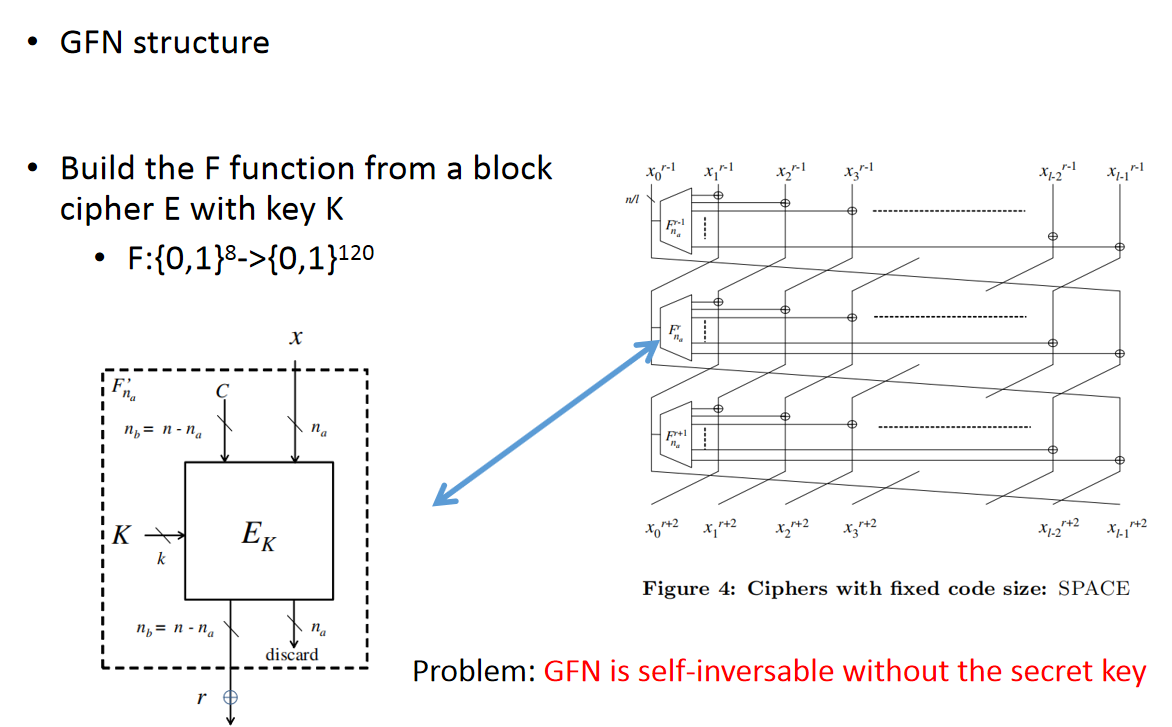
\includegraphics[width=8cm, height=5.5cm]{./pics/SPACE.png}};

    %\begin{scope}[x={(image.south east)},y={(image.north west)}]
        %\draw[help lines,xstep=.1,ystep=.1] (0,0) grid (1,1);
        %\foreach \x in {0,1,...,9} { \node [anchor=north] at (\x/10,0) {0.\x}; }
        %\foreach \y in {0,1,...,9} { \node [anchor=east] at (0,\y/10) {0.\y}; }
        %\draw[green, ultra thick, rounded corners] (0.24,0.18) rectangle (0.50,0.32);
    %\end{scope}
\end{tikzpicture}

\end{center}

}


\frame{
\frametitle{Space-hard ciphers:SPNBox}
In Asiacrypt 2016, Bogdanov and Isobe proposed \textcolor{red}{SPNBox}, which can be looked as the SPN version of SPACE.
\begin{center}
\begin{tikzpicture}
    \node[anchor=south west,inner sep=0] (image) at (0,0) { 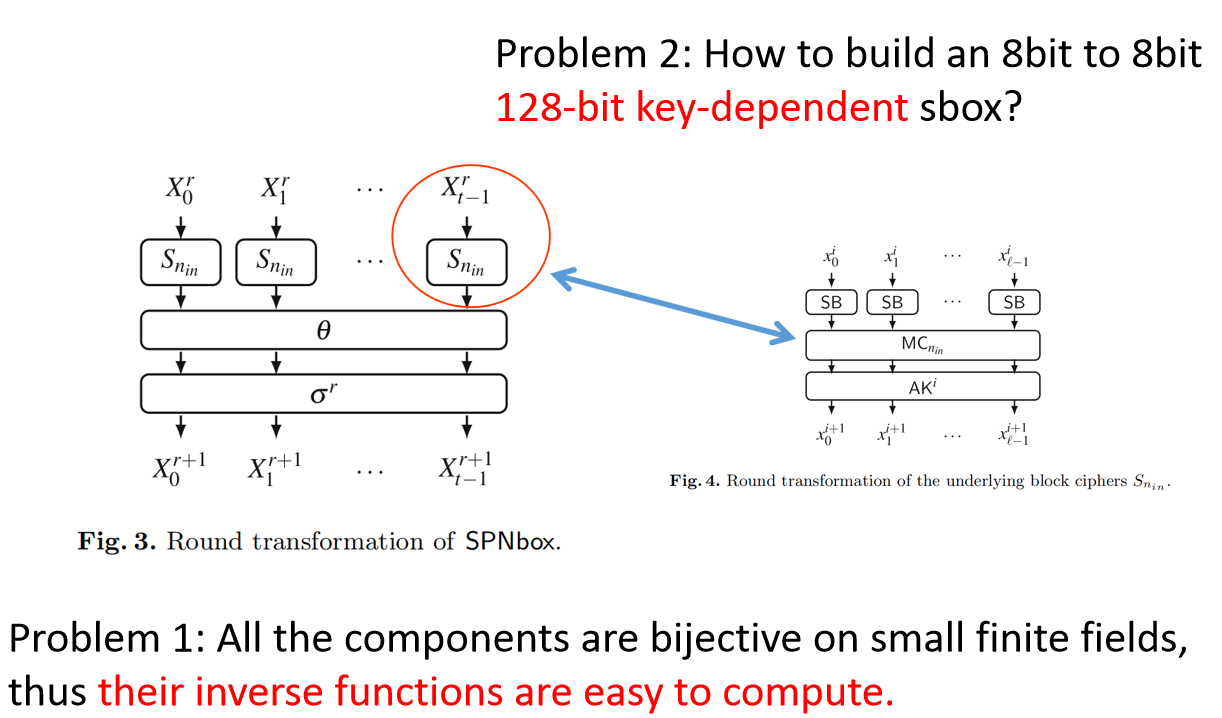
\includegraphics[width=8.5cm, height=5.5cm]{./pics/SPNBox.png}};

    %\begin{scope}[x={(image.south east)},y={(image.north west)}]
        %\draw[help lines,xstep=.1,ystep=.1] (0,0) grid (1,1);
        %\foreach \x in {0,1,...,9} { \node [anchor=north] at (\x/10,0) {0.\x}; }
        %\foreach \y in {0,1,...,9} { \node [anchor=east] at (0,\y/10) {0.\y}; }
        %\draw[green, ultra thick, rounded corners] (0.24,0.18) rectangle (0.50,0.32);
    %\end{scope}
\end{tikzpicture}

\end{center}

}

\frame
{
\frametitle{The problems of Space-hard ciphers}
\begin{itemize}
\item \textcolor{red}{Performance}: The costs of LUTs and computation are higher than CEJO-like constructions.\newline

\item \textcolor{red}{Weak WBC}: only achieves the weak white-box security (add encodings might be helpful but even worse on performance).

\item \textcolor{red}{Accuracy of space-hardness}: For example, if give 1000 bytes out of a 1024 bytes LUT, does attacker need to exhaustively search the remain 24 bytes?

\item \textcolor{red}{Compatibility}: only works for new designs (especially block ciphers).
\end{itemize}
}

\frame{
\frametitle{Bock \textit{et al.}'s white-box security with hardware/application-binding}
In Asiacrypt 2020 and CHES 2020, Bock \textit{et al.} proposed a white-box security key derivation function with \textcolor{red}{hardware/application-binding}, and then built a white-box payment application on it.

\begin{center}
\begin{tikzpicture}
    \node[anchor=south west,inner sep=0] (image) at (0,0) { 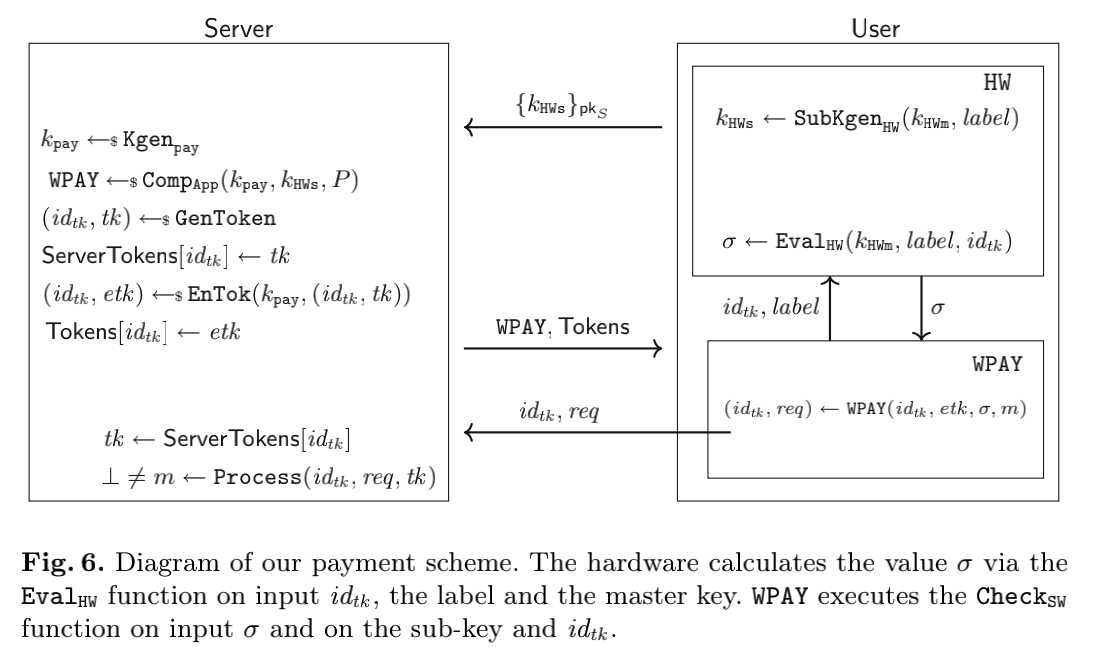
\includegraphics[width=8cm, height=5cm]{./pics/WKDF.png}};

    %\begin{scope}[x={(image.south east)},y={(image.north west)}]
        %\draw[help lines,xstep=.1,ystep=.1] (0,0) grid (1,1);
        %\foreach \x in {0,1,...,9} { \node [anchor=north] at (\x/10,0) {0.\x}; }
        %\foreach \y in {0,1,...,9} { \node [anchor=east] at (0,\y/10) {0.\y}; }
        %\draw[green, ultra thick, rounded corners] (0.24,0.18) rectangle (0.50,0.32);
    %\end{scope}
\end{tikzpicture}

\end{center}
}

\frame{
\frametitle{The problems of Bock \textit{et al.}'s hardware/application bound white-box security}
\begin{itemize}
\item It is not truly white-box security anymore if the precondition is a secure hardware. It becomes trusted computing.\newline

\item How to achieve hardware-binding is missing in the paper, the authors suggest using Android Keystore (which is insecure when it is rooted.)\newline

\item \textcolor{red}{If we already had a trusted hardware, why we need white-box cryptography? (e.g., using TEE is a better choice)}
\end{itemize}
}

\section{Our concerns on the security framework of WBC}
\subsection{The working range of WBC and its security framework}
\frame{
\frametitle{The practical perspective of white-box security}
Under the definitions of the black-box and the white-box securities, we propose a practical perspective of the white-box cryptography. The perspective is depicted from what the white-box cryptography can provide and how it should be secure against the adversary. Since the secret values are the most important in the white-box security model. A white-box cryptography can provide the following security properties.

\begin{itemize}
\item \textbf{Algorithm level: \textcolor{red}{Key recovery}.}

\item \textbf{Module level: Function integrity.}

\item \textbf{System level: Code lifting}

\end{itemize}
}

\frame{
\frametitle{}
Based on the above security properties that white-box cryptography could provide, one can build up secure applications enjoys the white-box security. From the life-cycle of secret keys, we depict the typical usages of the white-box cryptography in the following ways.

\begin{itemize}
\item \textbf{Key distribution.} Normally, the applications need a secure channel to distribute the secret keys between server and client. Although some key distribution schemes can be executed under authenticated channel, but most of them still need the support of certification services (Such as PKI, PKG, etc.). Because the white-box cryptography protects the secret keys from the adversary, the distribution of the keys only requires authenticated channel. If

\item \textbf{Local key management.}

\item \textbf{Dynamic key updating.}

\item \textbf{Key revocation.}
\end{itemize}
}

\frame{
\frametitle{}
For symmetric-key algorithms, they might be used for message authentication, data encryption/decrypiton and pseudorandom number generating. According to these different usages, the security requirements for the implementations of those cryptographic algorithms are diverse. Considering this diversity, we define a practical security notion for white-box cryptography as follows.

\begin{itemize}
\item \textbf{Key integrity.}

\item \textbf{Key confidentiality.}

\item \textbf{Key equivalence.}
\end{itemize}

}

\subsection{Adaptive DFA/DCA model and its application}
\frame
{
\frametitle{Adaptive DFA/DCA model}
\begin{itemize}
\setlength{\itemsep}{12pt}
\item The proposed DFA/DCA techniques are mainly in grey-box model.
\begin{itemize}
\setlength{\itemsep}{12pt}
\item The grey-box adversary does not know the details of WBC implementation.
\item Normally exploit with blind injection.
\item Some papers use reverse-engineering at first.
\end{itemize}

\item We assume a \textcolor{red}{greywhite}-box model.
\begin{itemize}
\setlength{\itemsep}{12pt}
\item The greywhite-box adversary still does not know the details of WBC implementation, but might know some parameters, e.g., rounds, sbox sizes.
\item Exploit with tweakable injection based on known parameters.
\item Avoid the reverse engineering.
\end{itemize}

\end{itemize}


}

\section{Conclusion}

\frame
{
\frametitle{Conclusion}

\begin{itemize}
\setlength{\itemsep}{12pt}
\item Security notions and definition for \textcolor{red}{precisely} analyze white-box cryptography are at very beginning.

\item Key protection definitions might not suitable in practice for non-key white-box applications, e.g., secure multi-party computation.

\item A secure white-box cryptography does not imply the white-box security of a secrecy system based on it.
\end{itemize}

}

\frame
{
\begin{center}
\textbf{Thanks for your attentions!}
\end{center}
\begin{center}
\begin{tikzpicture}
    \node[anchor=south west,inner sep=0] (image) at (0,0) { 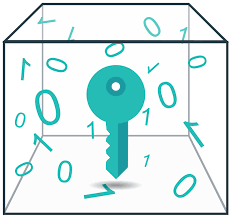
\includegraphics[width=4cm, height=4cm]{./pics/WBC_BG.png}};

    %\begin{scope}[x={(image.south east)},y={(image.north west)}]
        %\draw[help lines,xstep=.1,ystep=.1] (0,0) grid (1,1);
        %\foreach \x in {0,1,...,9} { \node [anchor=north] at (\x/10,0) {0.\x}; }
        %\foreach \y in {0,1,...,9} { \node [anchor=east] at (0,\y/10) {0.\y}; }
        %\draw[green, ultra thick, rounded corners] (0.24,0.18) rectangle (0.50,0.32);
    %\end{scope}
\end{tikzpicture}

\end{center}
}

\end{document}
